
%% bare_conf.tex
%% V1.3
%% 2007/01/11
%% by Michael Shell
%% See:
%% http://www.michaelshell.org/
%% for current contact information.
%%
%% This is a skeleton file demonstrating the use of IEEEtran.cls
%% (requires IEEEtran.cls version 1.7 or later) with an IEEE conference paper.
%%
%% Support sites:
%% http://www.michaelshell.org/tex/ieeetran/
%% http://www.ctan.org/tex-archive/macros/latex/contrib/IEEEtran/
%% and
%% http://www.ieee.org/

%%*************************************************************************
%% Legal Notice:
%% This code is offered as-is without any warranty either expressed or
%% implied; without even the implied warranty of MERCHANTABILITY or
%% FITNESS FOR A PARTICULAR PURPOSE! 
%% User assumes all risk.
%% In no event shall IEEE or any contributor to this code be liable for
%% any damages or losses, including, but not limited to, incidental,
%% consequential, or any other damages, resulting from the use or misuse
%% of any information contained here.
%%
%% All comments are the opinions of their respective authors and are not
%% necessarily endorsed by the IEEE.
%%
%% This work is distributed under the LaTeX Project Public License (LPPL)
%% ( http://www.latex-project.org/ ) version 1.3, and may be freely used,
%% distributed and modified. A copy of the LPPL, version 1.3, is included
%% in the base LaTeX documentation of all distributions of LaTeX released
%% 2003/12/01 or later.
%% Retain all contribution notices and credits.
%% ** Modified files should be clearly indicated as such, including  **
%% ** renaming them and changing author support contact information. **
%%
%% File list of work: IEEEtran.cls, IEEEtran_HOWTO.pdf, bare_adv.tex,
%%                    bare_conf.tex, bare_jrnl.tex, bare_jrnl_compsoc.tex
%%*************************************************************************

% *** Authors should verify (and, if needed, correct) their LaTeX system  ***
% *** with the testflow diagnostic prior to trusting their LaTeX platform ***
% *** with production work. IEEE's font choices can trigger bugs that do  ***
% *** not appear when using other class files.                            ***
% The testflow support page is at:
% http://www.michaelshell.org/tex/testflow/



% Note that the a4paper option is mainly intended so that authors in
% countries using A4 can easily print to A4 and see how their papers will
% look in print - the typesetting of the document will not typically be
% affected with changes in paper size (but the bottom and side margins will).
% Use the testflow package mentioned above to verify correct handling of
% both paper sizes by the user's LaTeX system.
%
% Also note that the "draftcls" or "draftclsnofoot", not "draft", option
% should be used if it is desired that the figures are to be displayed in
% draft mode.
%
\documentclass[conference]{IEEEtran}
\usepackage{blindtext, graphicx}
% Add the compsoc option for Computer Society conferences.
%
% If IEEEtran.cls has not been installed into the LaTeX system files,
% manually specify the path to it like:
% \documentclass[conference]{../sty/IEEEtran}





% Some very useful LaTeX packages include:
% (uncomment the ones you want to load)


% *** MISC UTILITY PACKAGES ***
%
%\usepackage{ifpdf}
% Heiko Oberdiek's ifpdf.sty is very useful if you need conditional
% compilation based on whether the output is pdf or dvi.
% usage:
% \ifpdf
%   % pdf code
% \else
%   % dvi code
% \fi
% The latest version of ifpdf.sty can be obtained from:
% http://www.ctan.org/tex-archive/macros/latex/contrib/oberdiek/
% Also, note that IEEEtran.cls V1.7 and later provides a builtin
% \ifCLASSINFOpdf conditional that works the same way.
% When switching from latex to pdflatex and vice-versa, the compiler may
% have to be run twice to clear warning/error messages.






% *** CITATION PACKAGES ***
%
%\usepackage{cite}
% cite.sty was written by Donald Arseneau
% V1.6 and later of IEEEtran pre-defines the format of the cite.sty package
% \cite{} output to follow that of IEEE. Loading the cite package will
% result in citation numbers being automatically sorted and properly
% "compressed/ranged". e.g., [1], [9], [2], [7], [5], [6] without using
% cite.sty will become [1], [2], [5]--[7], [9] using cite.sty. cite.sty's
% \cite will automatically add leading space, if needed. Use cite.sty's
% noadjust option (cite.sty V3.8 and later) if you want to turn this off.
% cite.sty is already installed on most LaTeX systems. Be sure and use
% version 4.0 (2003-05-27) and later if using hyperref.sty. cite.sty does
% not currently provide for hyperlinked citations.
% The latest version can be obtained at:
% http://www.ctan.org/tex-archive/macros/latex/contrib/cite/
% The documentation is contained in the cite.sty file itself.


\usepackage{algorithm}
\usepackage{algpseudocode}  
\usepackage{balance}

% *** GRAPHICS RELATED PACKAGES ***
%
\ifCLASSINFOpdf
  % \usepackage[pdftex]{graphicx}
  % declare the path(s) where your graphic files are
  % \graphicspath{{../pdf/}{../jpeg/}}
  % and their extensions so you won't have to specify these with
  % every instance of \includegraphics
  % \DeclareGraphicsExtensions{.pdf,.jpeg,.png}
\else
  % or other class option (dvipsone, dvipdf, if not using dvips). graphicx
  % will default to the driver specified in the system graphics.cfg if no
  % driver is specified.
  % \usepackage[dvips]{graphicx}
  % declare the path(s) where your graphic files are
  % \graphicspath{{../eps/}}
  % and their extensions so you won't have to specify these with
  % every instance of \includegraphics
  % \DeclareGraphicsExtensions{.eps}
\fi
% graphicx was written by David Carlisle and Sebastian Rahtz. It is
% required if you want graphics, photos, etc. graphicx.sty is already
% installed on most LaTeX systems. The latest version and documentation can
% be obtained at: 
% http://www.ctan.org/tex-archive/macros/latex/required/graphics/
% Another good source of documentation is "Using Imported Graphics in
% LaTeX2e" by Keith Reckdahl which can be found as epslatex.ps or
% epslatex.pdf at: http://www.ctan.org/tex-archive/info/
%
% latex, and pdflatex in dvi mode, support graphics in encapsulated
% postscript (.eps) format. pdflatex in pdf mode supports graphics
% in .pdf, .jpeg, .png and .mps (metapost) formats. Users should ensure
% that all non-photo figures use a vector format (.eps, .pdf, .mps) and
% not a bitmapped formats (.jpeg, .png). IEEE frowns on bitmapped formats
% which can result in "jaggedy"/blurry rendering of lines and letters as
% well as large increases in file sizes.
%
% You can find documentation about the pdfTeX application at:
% http://www.tug.org/applications/pdftex





% *** MATH PACKAGES ***
%
%\usepackage[cmex10]{amsmath}
% A popular package from the American Mathematical Society that provides
% many useful and powerful commands for dealing with mathematics. If using
% it, be sure to load this package with the cmex10 option to ensure that
% only type 1 fonts will utilized at all point sizes. Without this option,
% it is possible that some math symbols, particularly those within
% footnotes, will be rendered in bitmap form which will result in a
% document that can not be IEEE Xplore compliant!
%
% Also, note that the amsmath package sets \interdisplaylinepenalty to 10000
% thus preventing page breaks from occurring within multiline equations. Use:
%\interdisplaylinepenalty=2500
% after loading amsmath to restore such page breaks as IEEEtran.cls normally
% does. amsmath.sty is already installed on most LaTeX systems. The latest
% version and documentation can be obtained at:
% http://www.ctan.org/tex-archive/macros/latex/required/amslatex/math/





% *** SPECIALIZED LIST PACKAGES ***
%
%\usepackage{algorithmic}
% algorithmic.sty was written by Peter Williams and Rogerio Brito.
% This package provides an algorithmic environment fo describing algorithms.
% You can use the algorithmic environment in-text or within a figure
% environment to provide for a floating algorithm. Do NOT use the algorithm
% floating environment provided by algorithm.sty (by the same authors) or
% algorithm2e.sty (by Christophe Fiorio) as IEEE does not use dedicated
% algorithm float types and packages that provide these will not provide
% correct IEEE style captions. The latest version and documentation of
% algorithmic.sty can be obtained at:
% http://www.ctan.org/tex-archive/macros/latex/contrib/algorithms/
% There is also a support site at:
% http://algorithms.berlios.de/index.html
% Also of interest may be the (relatively newer and more customizable)
% algorithmicx.sty package by Szasz Janos:
% http://www.ctan.org/tex-archive/macros/latex/contrib/algorithmicx/




% *** ALIGNMENT PACKAGES ***
%
%\usepackage{array}
% Frank Mittelbach's and David Carlisle's array.sty patches and improves
% the standard LaTeX2e array and tabular environments to provide better
% appearance and additional user controls. As the default LaTeX2e table
% generation code is lacking to the point of almost being broken with
% respect to the quality of the end results, all users are strongly
% advised to use an enhanced (at the very least that provided by array.sty)
% set of table tools. array.sty is already installed on most systems. The
% latest version and documentation can be obtained at:
% http://www.ctan.org/tex-archive/macros/latex/required/tools/


%\usepackage{mdwmath}
%\usepackage{mdwtab}
% Also highly recommended is Mark Wooding's extremely powerful MDW tools,
% especially mdwmath.sty and mdwtab.sty which are used to format equations
% and tables, respectively. The MDWtools set is already installed on most
% LaTeX systems. The lastest version and documentation is available at:
% http://www.ctan.org/tex-archive/macros/latex/contrib/mdwtools/


% IEEEtran contains the IEEEeqnarray family of commands that can be used to
% generate multiline equations as well as matrices, tables, etc., of high
% quality.


%\usepackage{eqparbox}
% Also of notable interest is Scott Pakin's eqparbox package for creating
% (automatically sized) equal width boxes - aka "natural width parboxes".
% Available at:
% http://www.ctan.org/tex-archive/macros/latex/contrib/eqparbox/





% *** SUBFIGURE PACKAGES ***
%\usepackage[tight,footnotesize]{subfigure}
% subfigure.sty was written by Steven Douglas Cochran. This package makes it
% easy to put subfigures in your figures. e.g., "Figure 1a and 1b". For IEEE
% work, it is a good idea to load it with the tight package option to reduce
% the amount of white space around the subfigures. subfigure.sty is already
% installed on most LaTeX systems. The latest version and documentation can
% be obtained at:
% http://www.ctan.org/tex-archive/obsolete/macros/latex/contrib/subfigure/
% subfigure.sty has been superceeded by subfig.sty.



%\usepackage[caption=false]{caption}
%\usepackage[font=footnotesize]{subfig}
% subfig.sty, also written by Steven Douglas Cochran, is the modern
% replacement for subfigure.sty. However, subfig.sty requires and
% automatically loads Axel Sommerfeldt's caption.sty which will override
% IEEEtran.cls handling of captions and this will result in nonIEEE style
% figure/table captions. To prevent this problem, be sure and preload
% caption.sty with its "caption=false" package option. This is will preserve
% IEEEtran.cls handing of captions. Version 1.3 (2005/06/28) and later 
% (recommended due to many improvements over 1.2) of subfig.sty supports
% the caption=false option directly:
%\usepackage[caption=false,font=footnotesize]{subfig}
%
% The latest version and documentation can be obtained at:
% http://www.ctan.org/tex-archive/macros/latex/contrib/subfig/
% The latest version and documentation of caption.sty can be obtained at:
% http://www.ctan.org/tex-archive/macros/latex/contrib/caption/




% *** FLOAT PACKAGES ***
%
%\usepackage{fixltx2e}
% fixltx2e, the successor to the earlier fix2col.sty, was written by
% Frank Mittelbach and David Carlisle. This package corrects a few problems
% in the LaTeX2e kernel, the most notable of which is that in current
% LaTeX2e releases, the ordering of single and double column floats is not
% guaranteed to be preserved. Thus, an unpatched LaTeX2e can allow a
% single column figure to be placed prior to an earlier double column
% figure. The latest version and documentation can be found at:
% http://www.ctan.org/tex-archive/macros/latex/base/



%\usepackage{stfloats}
% stfloats.sty was written by Sigitas Tolusis. This package gives LaTeX2e
% the ability to do double column floats at the bottom of the page as well
% as the top. (e.g., "\begin{figure*}[!b]" is not normally possible in
% LaTeX2e). It also provides a command:
%\fnbelowfloat
% to enable the placement of footnotes below bottom floats (the standard
% LaTeX2e kernel puts them above bottom floats). This is an invasive package
% which rewrites many portions of the LaTeX2e float routines. It may not work
% with other packages that modify the LaTeX2e float routines. The latest
% version and documentation can be obtained at:
% http://www.ctan.org/tex-archive/macros/latex/contrib/sttools/
% Documentation is contained in the stfloats.sty comments as well as in the
% presfull.pdf file. Do not use the stfloats baselinefloat ability as IEEE
% does not allow \baselineskip to stretch. Authors submitting work to the
% IEEE should note that IEEE rarely uses double column equations and
% that authors should try to avoid such use. Do not be tempted to use the
% cuted.sty or midfloat.sty packages (also by Sigitas Tolusis) as IEEE does
% not format its papers in such ways.





% *** PDF, URL AND HYPERLINK PACKAGES ***
%
%\usepackage{url}
% url.sty was written by Donald Arseneau. It provides better support for
% handling and breaking URLs. url.sty is already installed on most LaTeX
% systems. The latest version can be obtained at:
% http://www.ctan.org/tex-archive/macros/latex/contrib/misc/
% Read the url.sty source comments for usage information. Basically,
% \url{my_url_here}.





% *** Do not adjust lengths that control margins, column widths, etc. ***
% *** Do not use packages that alter fonts (such as pslatex).         ***
% There should be no need to do such things with IEEEtran.cls V1.6 and later.
% (Unless specifically asked to do so by the journal or conference you plan
% to submit to, of course. )


% correct bad hyphenation here
\hyphenation{op-tical net-works semi-conduc-tor}


\begin{document}
%
% paper title
% can use linebreaks \\ within to get better formatting as desired
\title{Anatomy of machine learning algorithm implementations
in MPI, Spark, and Flink}


% author names and affiliations
% use a multiple column layout for up to three different
% affiliations
% \author{\IEEEauthorblockN{Supun Kamburugamuve, Pulasthi Wickramasinghe, Geoffrey C. Fox}
% \IEEEauthorblockA{School of Informatics and Computing\\
% Indiana University, Bloomington\\
% skamburu@indiana.edu, pswickra@indiana.edu, sekanaya@indiana.edu, gcf@indiana.edu}
% \and
% \IEEEauthorblockN{Saliya Ekanayake}
% \IEEEauthorblockA{Network Dynamics and Simulation Science Laboratory\\
% Biocomplexity Institute, Virginia Tech, Blacksburg, VA\\
% esaliya@vt.edu}
% }

\author{
    \IEEEauthorblockN{Supun Kamburugamuve\IEEEauthorrefmark{1}, Pulasthi Wickramasinghe\IEEEauthorrefmark{1}, Saliya Ekanayake\IEEEauthorrefmark{2}, Geoffrey C. Fox\IEEEauthorrefmark{1}}
    \IEEEauthorblockA{\IEEEauthorrefmark{1}School of Informatics and Computing\\
Indiana University, Bloomington
    \\\{skamburu, pswickra, gcf\}@indiana.edu}
    \IEEEauthorblockA{\IEEEauthorrefmark{2} Network Dynamics and Simulation Science Laboratory \\ Biocomplexity Institute, Virginia Tech, Blacksburg, VA
    \\\{esaliya\}@vt.edu}
}
% conference papers do not typically use \thanks and this command
% is locked out in conference mode. If really needed, such as for
% the acknowledgment of grants, issue a \IEEEoverridecommandlockouts
% after \documentclass

% for over three affiliations, or if they all won't fit within the width
% of the page, use this alternative format:
% 
%\author{\IEEEauthorblockN{Michael Shell\IEEEauthorrefmark{1},
%Homer Simpson\IEEEauthorrefmark{2},
%James Kirk\IEEEauthorrefmark{3}, 
%Montgomery Scott\IEEEauthorrefmark{3} and
%Eldon Tyrell\IEEEauthorrefmark{4}}
%\IEEEauthorblockA{\IEEEauthorrefmark{1}School of Electrical and Computer Engineering\\
%Georgia Institute of Technology,
%Atlanta, Georgia 30332--0250\\ Email: see http://www.michaelshell.org/contact.html}
%\IEEEauthorblockA{\IEEEauthorrefmark{2}Twentieth Century Fox, Springfield, USA\\
%Email: homer@thesimpsons.com}
%\IEEEauthorblockA{\IEEEauthorrefmark{3}Starfleet Academy, San Francisco, California 96678-2391\\
%Telephone: (800) 555--1212, Fax: (888) 555--1212}
%\IEEEauthorblockA{\IEEEauthorrefmark{4}Tyrell Inc., 123 Replicant Street, Los Angeles, California 90210--4321}}




% use for special paper notices
%\IEEEspecialpapernotice{(Invited Paper)}




% make the title area
\maketitle


\begin{abstract}
With the ever-increasing need to analyze large amounts of data to get useful insights, it is essential to develop complex parallel machine learning algorithms that can scale with data and number of parallel processes. These algorithms need to run on large data sets as well as they need to be executed with minimal time in order to extract useful information in a time constrained environment. MPI is a widely used model for developing such algorithms in high-performance computing paradigm while Apache Spark and Apache Flink are emerging as big data platforms for large-scale parallel machine learning. Even though these big data frameworks are designed differently, they follow the data flow model for execution and user APIs. Data flow model offers fundamentally different capabilities than the MPI execution model, but the same type of parallelism can be used in applications developed in both models. This paper presents three distinct machine learning algorithms implemented in MPI, Spark, and Flink and compares their performance and identifies strengths and weaknesses in each platform. 

%By doing so the paper identifies the similarities and differences between big data platforms and MPI execution model for large scale data analytics.  

%With the ever-increasing need to analyze large amounts of data to get useful insights, it is essential to develop complex parallel machine learning algorithms that can scale with data and numbers of parallel processes. These algorithms should be able to run on large data sets as well as they need to be executed with minimal time in order to give useful information to the public. MPI is a widely used model for developing such algorithms in high performance computing paradigm while Apache Spark and Apache Flink are emerging as big data platforms for doing large-scale parallel machine learning. Big data tools use different approaches and execution models during run time which makes each tool different from other. Each has their own weaknesses and strengths.  In this paper we present three distinct machine learning algorithms implemented in MPI, Spark and Flink and compare their strengths and weaknesses.
%
\end{abstract}
% IEEEtran.cls defaults to using nonbold math in the Abstract.
% This preserves the distinction between vectors and scalars. However,
% if the journal you are submitting to favors bold math in the abstract,
% then you can use LaTeX's standard command \boldmath at the very start
% of the abstract to achieve this. Many IEEE journals frown on math
% in the abstract anyway.

% Note that keywords are not normally used for peerreview papers.
\begin{IEEEkeywords}
Machine Learning, Big data, HPC, MDS, MPI, Spark, Flink, K-Means, Terasort
\end{IEEEkeywords}






% For peer review papers, you can put extra information on the cover
% page as needed:
% \ifCLASSOPTIONpeerreview
% \begin{center} \bfseries EDICS Category: 3-BBND \end{center}
% \fi
%
% For peerreview papers, this IEEEtran command inserts a page break and
% creates the second title. It will be ignored for other modes.
\IEEEpeerreviewmaketitle



\section{Introduction}
Machine learning algorithms are increasingly popular for handling large-scale data analytics. With the prevailing era of tremendous data sizes and complex algorithms, it is necessary to use parallel computing to make these algorithms compute in a reasonable amount of time. There are many frameworks available to run such algorithms in parallel from the High performance computing (HPC) and Big Data communities. Message passing interface(MPI) is the most widely used and dominant technology in HPC for parallel data analytics. Numerous frameworks exist in the Big Data community for doing large-scale parallel computations for machine learning algorithms, including Hadoop~\cite{White:2009:HDG:1717298}, Spark~\cite{Zaharia:2010:SCC:1863103.1863113}, Flink~\cite{apache_flink, carbone2015lightweight}, Tez~\cite{saha2015apache} and Google Dataflow~\cite{akidau2015dataflow}, and it is worthwhile to note there is no single technology that stands out among others as the best. 

Hadoop is an early big data system for analyzing very large data sets. It employed a limited data flow API with map and reduce functions to move data and do computations. Later on it became clear that Hadoop was not efficient enough for the majority of Big Data problems, especially machine learning applications involving iterative computations~\cite{Ekanayake:2010:TRI:1851476.1851593}. Spark, Flink and Tez are some of the later systems that overcame these bottlenecks. They expose richer data flow APIs along with in-memory computations and iterative computing support to be much more efficient than Hadoop.

MPI programming API utilises an in-memory in-place execution model where the computations and communications both happen in the same process under the same programming scope. On the other hand, Big Data systems have adopted a data flow style programming model and execution model for processing large amounts of data. Both Flink and Spark feature data flow APIs, and their execution also happens in data flow style. In Data-flow programming model, operators are applied on distributed data sets which produce other distributed data sets. This abstraction provides a simple yet very powerful programming API. These APIs are usually written in accordance with the functional programming principles, making them less error prone and easy to program. A data-flow execution model separates the communications and computations by allowing computing to happen in self-contained tasks and not permitting communication within the task execution. The tasks do stateless computations on the data. 

In contrast to these high level programming APIs, MPI provides bare communication primitives necessary for parallel computing. The MPI primitives are highly optimized for HPC environments with primary focus on in-memory stateful computing and support for advanced hardware such as high performance interconnects. With recent trends in the Big Data community, we see Big Data frameworks are inclined to use some of the hardware and algorithmic advances applied in traditional HPC frameworks. Even though MPI is a generic programming API, it is harder to use than Spark or Flink style programs without using substantial programming. 

Among the big data frameworks we have mentioned earlier, Apache Flink and Spark are popular and efficient examples. These two have been used heavily in machine learning applications owing to having personalize machine learning libraries called FlinkML~\cite{carbone2015lightweight} and MLib~\cite{meng2016mllib}, respectively. Because of the in-memory nature of the computations, we can argue that MPI, Flink and Spark provide a comparable feature set for machine learning applications. Even though these frameworks have been positioned as enablers of large-scale machine learning, it is hard to find complex machine learning algorithms with heavy computational and communication demands implemented in these platforms. 

This paper examines three distinctively different algorithms implemented in Spark, Flink and MPI and studies their performance characteristics. The algorithms discussed here are Multidimensional Scaling~\cite{kruskal1964multidimensional}, K-Means and Terabyte sort. We compare the two contrasting styles of programming and execution models offered by Big Data frameworks and MPI to point out the advantages and disadvantages of both approaches for parallel machine learning applications. Furthermore, the paper analyzes the algorithms on all three platforms and draws a clear distinction between the strengths and weaknesses of the frameworks.

The rest of the paper is organized as follows. Section~\ref{data_flow_mpi} describes the data flow and MPI models of computation along with background information about Spark and Flink. Section~\ref{mds}~\ref{kmeans}~\ref{terasort} explains the MDS, K-Means and Terasort algorithms respectively and explains their implementations in Spark, Flink and MPI. The next Section~\ref{evaluation} describes the experiments conducted while Section~\ref{discussion} explains the results observed. Related work is discussed in Section~\ref{related} and the paper concludes in Section~\ref{conclusion}.

\section{Data flow and MPI} \label{data_flow_mpi}

\subsection{Execution models}

Data flow frameworks model computation as a graph where nodes represent the operators that are applied to data and edges represent the communication channels between the operators. The input and output of an operator is sent through the edges. Operators are user defined code that execute on the data and produce other data. The graph is created using data flow functions provided by the framework. These data flow functions act upon the data to create the graph. An example function is a partition function, often called a map in data flow engines. A map function works on partitions of a data set and presents the partitioned data to the user defined operators at the nodes. The output of a user defined operator is connected to another user defined operator using a data flow function. Map and reduce are such two widely used data flow functions. 

The data flow model consist of a logical graph and an execution graph. The logical graph is defined by the user with data, data flow functions and user operators. The execution graph is created by the framework to deploy the logical graph on the cluster. For example, some user functions may run in larger numbers of nodes depending on the user defined parallelism and size of input. Also when creating the execution graph the framework can apply optimizations to make some data flow operations more efficient. An example logical graph is shown in Fig.~\ref{fig:logical_graph} where it displays a map and reduce data flow functions. Fig.~\ref{fig:execution_graph} shows an execution graph for this logical graph where it runs multiple map operations and reduce operations in parallel. It is worth noting that each user defined function runs on its own program scope without access to any state about previous tasks. The only way to communicate between tasks is using messaging, as tasks can run in different places.

For task execution, frameworks use a thread model with fewer task managers executing the parallel tasks for a node. This leads to a smaller number of TCP connections between the nodes, but the individual tasks are subjected to interference by other task executions. 

\begin{figure}
    \centering
    
\includegraphics[width=0.95\columnwidth]{images/logical_graph.png}
    \caption{Logical graph of a data flow}
    \label{fig:logical_graph}
\end{figure}

\begin{figure}
    \centering
    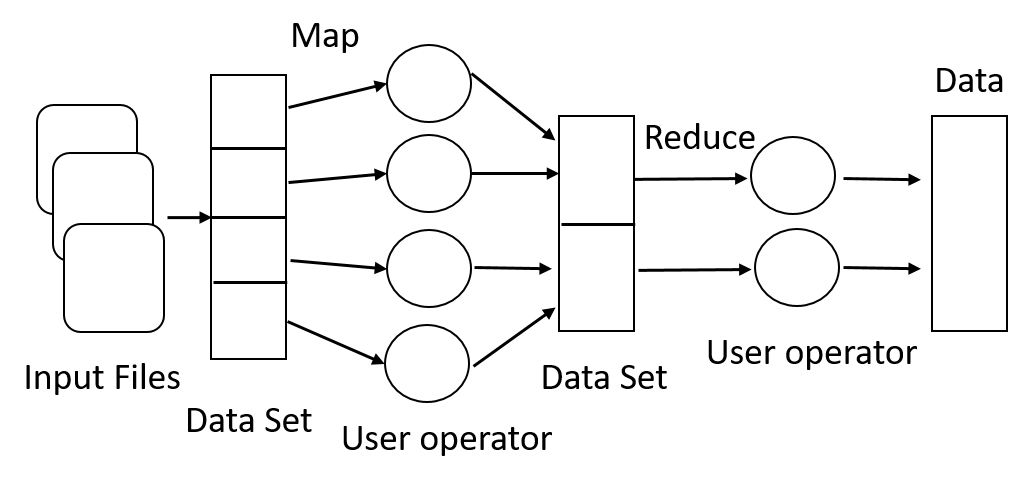
\includegraphics[width=0.95\columnwidth]{images/execution_graphs.png}
    \caption{Execution graph of a data flow}
    \label{fig:execution_graph}
\end{figure}

Message passing interface (MPI) is a generic model for doing parallel computations. It is used most widely in the single program multiple data (SPMD) style of parallel programs. The parallel processes can employ MPI functions for both message passing and synchronization between the processes. Fig.~\ref{fig:execution_graph} shows the execution model of MPI. Unlike in data flow, the same process does the communion and computations throughout the execution. The processes are normal Unix versions spawned by MPI. 

\begin{figure}
    \centering
    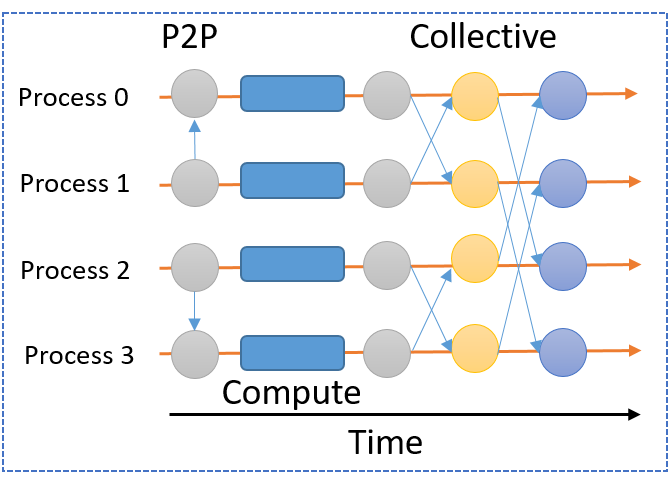
\includegraphics[width=0.7\columnwidth]{images/mpi-flow.png}
    \caption{Execution flow of MPI program with compute and communication regions}
    \label{fig:execution_graph}
\end{figure}

\subsection{Programming APIs}

Popular data flow engines such as Spark, Flink and Google Data Flow all enable a functional programming API. The data is abstracted as high level language objects. A large distributed data set is represented as a programming construct. For example, in Flink the data structure is called a DataSet, while in Spark it is a RDD. These data sets are considered immutable, meaning they cannot be changed once created. 

The user defined operators are implemented according to the functional programming paradigm with no side effects, meaning a user defined code cannot modify out-of-scope data sets or passed-in data sets. The only way an operator can produce a new data set is by outputting it, thus creating a different version every time. This clean programming paradigm makes it easier for an average programmer to write data-flow programs faster and error-free. But it comes with the cost of creating new structures every time a data set has to be modified. In MPI style programs, we almost always modify the existing memory structures without producing new data sets every time a small operation is applied to the data. The data flow functions are always applied to these data objects. Usually a data flow function implements a user defined function to act upon the data it receives, although there are functions that don't accept user defined programs.

The data loading and data saving is abstracted out in terms of data sources and sinks. Data source and sinks are responsible for reading and writing the data while hiding the details of different file systems such as local file systems and distributed file systems like HDFS. The default data sources are sufficient for large sets of applications but for more advanced use cases users often end up writing their own readers and writers. 

\subsection{Apache Flink}

Apache Flink is a batch and stream processing engine that models every computation as a data flow graph which is then submitted to the Flink cluster. The nodes in this graph are the computations and the edges are the communication links. Flink closely resembles the both the data flow execution model and API. The user graph is transformed into an execution graph by Flink before it is executed on the distributed nodes. While undergoing this transformation, Flink optimizes the user graph, taking into account the data locality. Flink uses and thread based worker model for executing the data flow graphs. It can chain consecutive tasks in the work flow in a single node to make the run more efficient by reducing data serializations and communications.

Even though Flink has a nice theoretically sound data flow abstraction for programming, we found that it is difficult to program in a strictly data-flow fashion for complex programs. This primarily due to the fact that control flow operations such as if conditions and iterations are harder code in data flow paradigm.

\subsection{Apache Spark}

Apache Spark is a distributed in-memory data processing engine. The data model in Spark is based around RDDs~\cite{zaharia2012resilient}, and the execution model is based on RDDs and lineage graphs. The lineage graph captures dependencies between RDDs and their transformations. The logical execution model is expressed through a chain of transformations on RDDs by the user. This lineage graph is also essential in supporting fault tolerance in Apache Spark.

RDD's can be read in from a file system such as HDFS, and transformations are applied to the RDDs. Spark transformations are lazy operations and actual work is only done when an action operation such as count, reduce are invoked. By default, intermediate RDDs created through transformations are not cached and will be recomputed when needed. The user has the ability to cache or persist intermediate RDDs by specifying this explicitly. This is very important for iterative computation where same data sets are being used over and over again.  

Spark primarily uses an thread based worker model for executing the tasks. Unlike in Flink where user submits the execution graph to the engine, Spark programs are controlled by a driver program. This driver program usually runs in a separate master node and the parallel regions in this driver program are shipped to the cluster to be executed. With this model complex control flow operations that needs to run serially such as iterations and if conditions run in master while data flow operators are executed in worker nodes. While this model makes it easier to write complex programs, it is harder to do complex optimizations on the data flow graph as it needs to be executed on the fly.

\section{Multidimensional Scaling} \label{mds}

Multidimensional scaling is a popular, well established machine learning technique for projecting high dimensional data into a lower dimension so that they can be analyzed. It has been extensively used to visualize high dimensional data by projecting into 3D or 2D models. MDS is a computationally expensive algorithm. The best algorithms are in the range of $O(N^2)$. When applied to a larger data set, the computation time increases exponentially. The algorithm can be made to run efficiently in parallel to reduce the computation time requirements. 

Parallel version of MDS requires multiple parallel regions and nested iterations for its computations. We will not go through the details of the algorithm as it is already described in several previous works~\cite{DBLP:conf/eScience/RuanF13,hpc2016:spidaljava, ekanayakejava}. The initial work~\cite{DBLP:conf/eScience/RuanF13} illustrates how the original MDS algorithms complexity is being lowered from $O(N^3)$ to $O(N^2)$. The proceeding papers~\cite{hpc2016:spidaljava,ekanayakejava} describe techniques for improving the implementation efficiency using Java and MPI. For the purpose of this study we only investigate the algorithm in terms of parallel operations it requires, their complexity and how they can be run in parallel as we try to analyze this algorithm on three execution platforms.

Given a high dimensional distance matrix, the goal of MDS algorithm is to produce a point file with the target dimension. Optionally the algorithm can take a weight matrix. The flow of the algorithm is shown in flow diagram~\ref{fig:fig_damds_flow}. MDS algorithm begins by reading two files which contain the pair of matrices. If the data set has $N$ high dimensional data points, the size of these matrices will be $N \times N$ with each cell containing 2 bytes of data in the form of a Short Integer. One matrix file contains the distances and the other contains the weights. Each worker in the computation only reads part of the $N \times N$ matrix. Aside from these two matrices, the algorithm requires a $N \times  M$ matrix where $M$ is the target projection dimension. In most cases $M$ will be 3 or 2. 

The pseudo code of the algorithm is shown in~\ref{mds_code} emphasizing on the important parallel operations. Since this particular implementation of MDS uses deterministic annealing(DA) as an optimization technique, the algorithm has an outer loop involving temperature. The temperature is lowered after each loop until it reaches a configured low value. For each degree reading, the solution to the MDS equation is found as an optimization. For each iteration, the stress is lowered until the difference between consecutive stresses are minimal enough. This involves the last two loops, where the middle loop is over stress and the inner loop is for the optimization computation.

The core of the computation involves several matrix multiplications. The remaining computations are mainly serial in nature. These matrix multiplications are present in the two inner loops and largely involve $N \times N$ into $N \times M$ matrices. The algorithm is made parallel around these matrix multiplications.

\begin{algorithm}
\caption{MDS Parallel operations}
\label{mds_code}
\small
    \begin{algorithmic}[1]
      \State $d,w_i,P,n,m$ \Comment{Where d - partition of D, w - partition of W, p - Initial points, N -  number of points, M - target dimension, K - number of parallel tasks}
        \State{$P = [N,M] $}\ point matrix
        \State{$b = $ $N \over K$}
        \State{$d = [b,N]$} \ partition of D matrix
        \State{$w = [b,N]$} \ partition of W matrix
        \State{$BC =[N,M]$} \ NxM matrix   
        \State{$V =[b]$} \ Array
        \State{$T$} \ DA temperature
       
       \While{$T > 0$}
            \State $preStress = calculateStress(d,w,P,T)$            
            \While{$stressDiff > delta$} 
                \State $BC = calculateBC(d,w,P,T)$   
                \State $P = conjugateGradient(d,w,P,T,BC)$
                \State $stress = calculateStress(d,w,P,T)$
                \State $stressDiff = preStress - stress$
                \State $preStress = stress $
            \EndWhile  
            \State $T = \alpha \time T$
       \EndWhile
       
       \Function{conjugateGradient}{$d,w,P,T,BC$}
            \State{$MMr =[N,M]$} \ NxM matrix
            \State $MMr = calculateMM(w,V,P)$ 
            \State $BC = BC - MMr$
            \State $MMr = BC$
            \State $rTr = innerProduct(MMr,MMr)$
            \State $testEnd = rTr * cgThreshold$
            \While{$itr < cgCount$}
                \State $MMAp = calculateMM(w,V,BC)$
                \State $\alpha = rTr/innerProduct(BC,MMAp)$
                \State $P = P + \alpha * BC$
                \If{$rTr < testEnd$}
                    \State break
                \EndIf
                \State $MMr = MMr - \alpha * MMAp$
                \State $temp = innerProduct(MMr,MMr)$
                \State $\beta = temp/rTr$
                \State $rTr = temp$
                \State $BC = MMr + \beta * BC$
            \EndWhile
            \State return $P$         
       \EndFunction    
       
       \Function{calculateStress}{$d,w,P,T$} \Comment{parallel operation}
            \State calculate partial value of Stress (Double value) 
            \State All Reduce partial stress (sum) 
            \State {return $stress$}
       \EndFunction    
       
       \Function{calculateBC}{$d,w,P,T$} \Comment{parallel operation}
            \State calculate partial value of BC for $[b,M]$ matrix 
            \State gather the other parts from peers (AllGather)
            \State {return $BC$}
       \EndFunction    
       
        \Function{calculateMM}{$w,V,A$} \Comment{parallel operation}
            \State calculate $wA$ using $V$ for diagnol values of $w$
            \State AllGather $[b,M]$ parts from peers
            \State return the collected $[N,M]$ matrix
        \EndFunction
       \Function{innerProduct}{$A,B$}
            \State return sum of vector dot products
       \EndFunction
\end{algorithmic}
\end{algorithm}

\begin{figure}
    \centering
    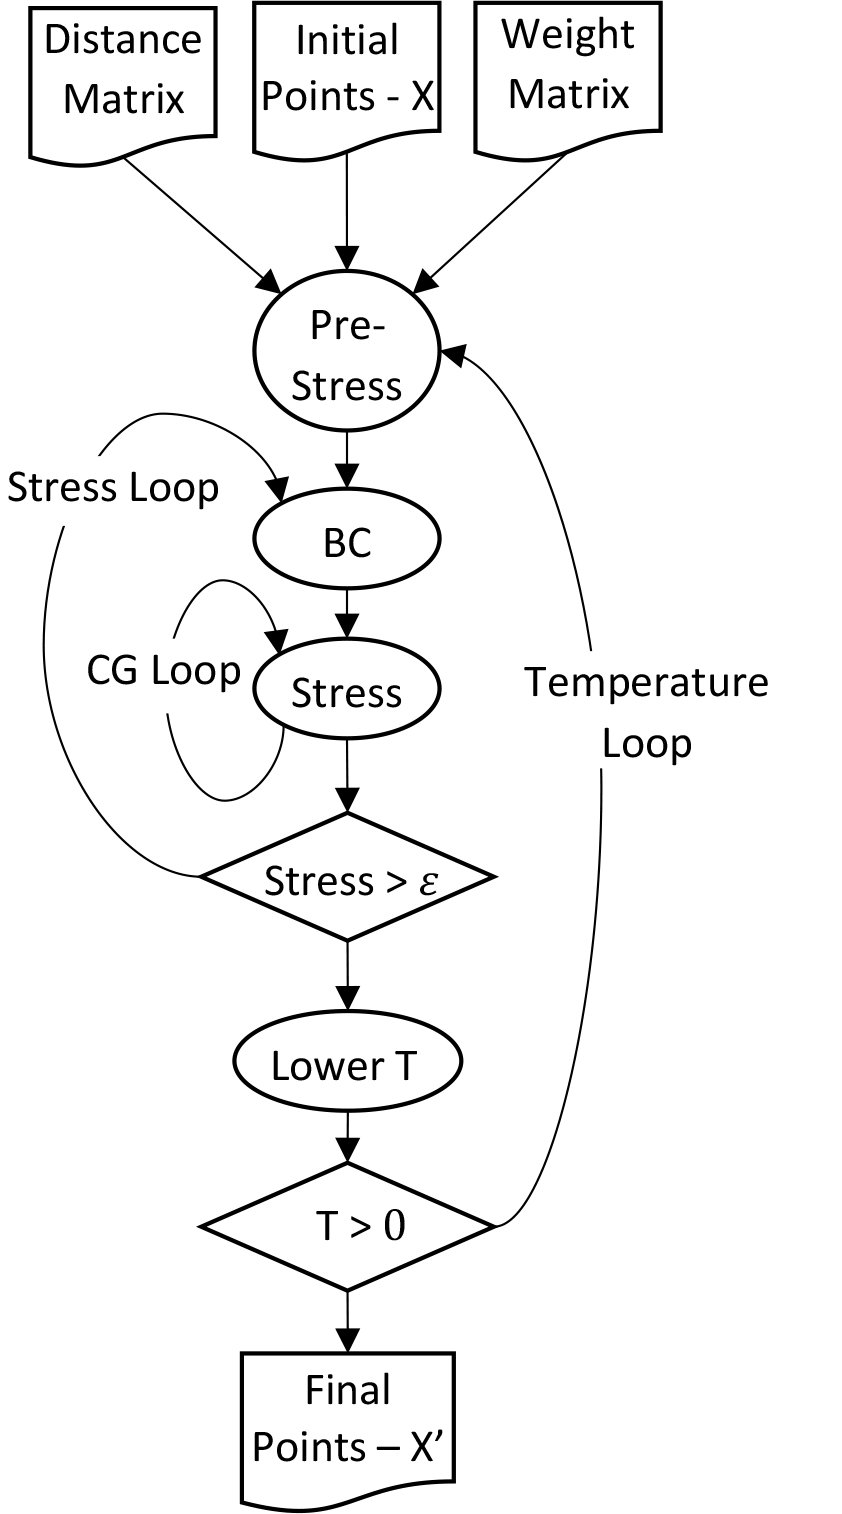
\includegraphics[width=0.5\columnwidth]{images/damds.png}
    \caption{Multidimensional Scaling algorithm with Deterministic Annealing control flow}
    \label{fig:fig_damds_flow}
\end{figure}

Apart from the 3 matrices already described, three other matrix of size $N \times M$ are required, called $BC$,$MMr$ and $MMa$ and one array $V$ of size $N$. For this algorithm we can achieve a balanced load across the parallel workers. The two $N \time N$ matrices read are partitioned row-wise. The $N \times M$ matrix, which contains the projected points, is maintained as a whole in all the workers along with along with $BC$,$MMr$ and $MMa$. 

\subsection{MPI Implementation}

The MPI implementation is a BSP style program written in Java using the OpenMPI Java bindings. Computations in DA-MDS grow $O(N^2)$ and communications $O(N)$. The algorithm involves gather/reduce of large matrices. Because of this the communication between the workers is very intensive. The MPI implementation uses shared memory explicitly to reduce the cost of collective operations by doing local operation to a node first before doing the global collective operation. The MPI implementation is further enhanced with different styles of threads to utilize the modern multi-core machines. 

\subsection{Apache Flink Implementation}

Flink starts the implementation with custom input formats for reading the binary matrix files and text based point files required by MDS. Compared to MPI implementation it was much easier to deal with the high level APIs of the input format for handling data partitioning and reading. The parallel operations in the MDS algorithm are mostly implemented using Map, Reduce and GroupReduce operations in Flink API. Also the broadcast functionality is used heavily throughout the program.

As of this work, Flink doesn't support nested iterations and only supports single level iterations. Because of this limitation, only the last loop is implemented as a data-flow. To handle the two outer loops, the implementation used separate jobs. As such each job executes the innermost loop and saves the computation to disk. Then the next outer loop starts as a new job with the saved state. This is a very inefficient way of implementing the iterations because Flink has to schedule the job, load data and save intermediate data for each of the two outer loops. We noticed that data loading doesn't add much overhead, but scheduling the tasks does.

Flink does not support outputting variables created inside an iteration. This leads to the creation of unified data sets with both the loop variable and output variable in a single data set. Because of this we had to pass these two data sets to distributed operations that only handle one of them at a time. Flink has no mechanism to load the same data set over all the workers and maintain such structures across all the nodes throughout different data flow operations. So the point matrix is created only in a single node. Every time there is a parallel operation requiring the point matrix, it has to be broadcast to the workers. This applies to other matrices such as BC and MMr as well.

The data flow operators are scheduled by Flink without much control from the user about where to place the data and operators in a cluster. For a complex data flow application such as MDS, it is important to have some control over where the data and operators are placed in the cluster while doing the computation to apply many application-specific optimizations. For simple data flow application, this gives a perfect abstraction and an easy API for users to write efficient programs. But for complex applications it may not translate well as in the easy case. Also it is worth noting that, Flink has to model the serial operation in the algorithm according to the data flow style.

Even though Flink programming model can become complex and non-intuitive for complex algorithms, we found that the programs were surprisingly free of programming errors compared to MPI programs. This is primarily due to the functional style of programming API where user cannot change state. 
 
\subsection{Spark Implementation}

The programming model of Spark does not allow tasks to communicate with one another, therefore all-to-all collectives are not supported in Spark. As a result, at each iteration the data needs to be collected at the master process and then a new set of tasks has to be created with the new data for the next iteration. This adds two additional overheads to the algorithm. The first is task creation and distribution at each iteration. The other is caused by the additional I/O that needs to be done at each step to perform reduce and broadcast instead of an AllReduce operation. Because of these limitations the main loops of the MDS algorithm are executed in the driver program and large tasks such as calculateBC, calculateMM and calculateStress are performed as distributed map-reduce tasks. This results in a large number of map reduce phases. The resulting values are then broadcast from the driver program to the cluster before the next iteration is executed. Several RDD's that contain distance data and weight data are cached to improve performance. 

Because Spark does not allow in-place changes on RDDs, the algorithm generates intermediate data sets that are not required in the MPI implementation. These intermediate data sets increase the memory usage of the algorithm, which is problematic because memory is a limiting factor when running MDS on very large matrices.

\section{K-Means algorithm} \label{kmeans}

K-Means is an efficient and practical classical machine learning algorithm for data clustering. The algorithm maintains K cluster points called centroids. There are many variations of K-means available, but for these experiments we use the simplest form. As described in the pseudo code~\ref{kmeans_algo}, parallel algorithm works as follows: the input to the system is $N$ points and $K$ initial centroids generated randomly. The $N$ points are partitioned among the parallel tasks and each parallel processes read the $K$ initial centroids. After this step, every task calculates its nearest centroid for each point. The local average of these points for each centroid are used in a global average to get the new centroids position. This is essentially an AllReduce operation with sum. 

\begin{figure}
    \centering
    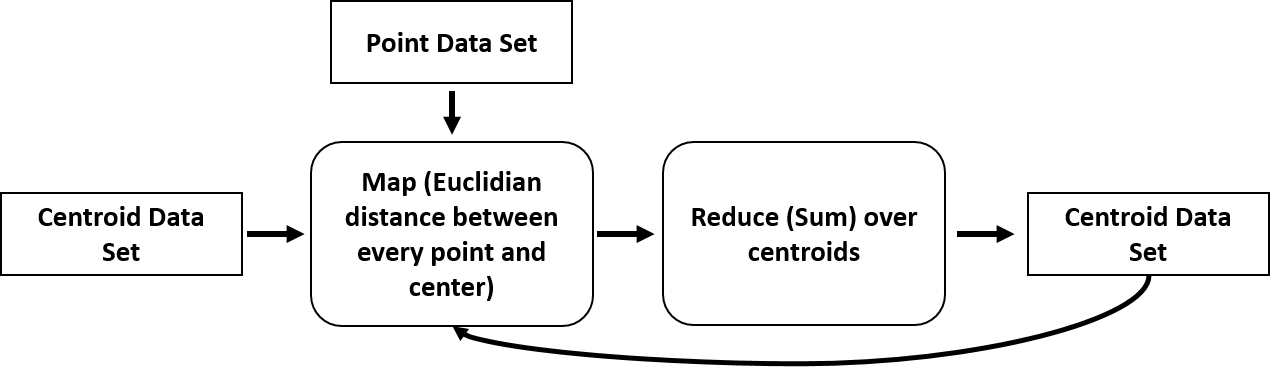
\includegraphics[width=0.95\columnwidth]{images/k-means.png}
    \caption{K-Means data flow graph for Flink and Spark}
    \label{fig:fig_k_means_flow}
\end{figure}

\subsection{MPI Implementation}

Each parallel MPI implementation reads its partition of the point data set and calculates the nearest centroid for each point. The average of these local values are summed over all the ranks using the MPI AllReduce operation to find the new centroids.

\subsection{Spark \& Flink Implementations}

Spark and Flink K-Means data flow graph is shown in Fig~\ref{fig:fig_k_means_flow}. At each iteration, a new set of centroids are calculated and fed back to the beginning of the iteration. The algorithm partitions the points into multiple map tasks and uses the full set of centroids in every one. Each map task assigns its points to their nearest centroid. The average of points is reduced (sum) for each centroid to get the new set of centroids, which are broadcast to the next iteration. Spark MLib provides a implementation of K-Means, which is used for evaluations. 

In MPI after the AllReduce operation, the centroids are updated within the program in-place. On the other hand, for Spark and Flink these centroids need to be broadcast back to all the tasks that do the nearest neighbor calculation in the next iteration. We can argue that all reduce operation in MPI is equivalent to reduce + broadcast, which is the mechanism used in Flink and Spark. But it is worth noting that AllReduce can be optimized for greater efficiency than running reduce and broadcast separately by using algorithms such as recursive doubling.

\section{Terasort} \label{terasort}

Sorting terabytes of data is a utility algorithm used by larger machine learning applications. The algorithm itself presents some interesting characteristics when we compare with MPI and data flow style applications. Spark, Flink and MPI implementations of the algorithm use the strategy shown in Fig~\ref{fig:tera_shuffle} to sort 1 terabyte of data in parallel. At the initial stage, the data is partitioned into equal size chunks among the processes. The processes load these chunks into memory and uses a sample set of data to find an ordered partitioning of the global data set. It does this by sorting the samples gathered from a configurable number of processes. Given that the data is well balanced and the number of sample partitions are reasonably high, this step normally generates a balanced partitioning of the data. In the next step, this global partitioning is used by all the processes to send the data to the correct parallel task. We call this the shuffling phase. The parallel version of the algorithm is described in code~\ref{tearasort_algo}. After a process receives the data it requires from other processes, it sorts and writes them to a file. This creates a globally sorted data set across the parallel tasks. 

\begin{algorithm}
   \caption{Parallel K-Means algorithm}
   \footnotesize
   \label{kmeans_algo}
    \begin{algorithmic}[1]
    \State $W$ number of parallel processes
    \State $P$ point partition
    \State $C$ initial centers 
    \State $C_1 = C$    
    \For{$i = 1$ to $iterations$}
        \State $C_{i+1} = 0$ next set of centers
        \For{$p = $ in $P$}
            \State Calculate the nearest center $i$ for $p$ in $C_{i}$        
            \State add $p$ to the $i$ center in $C_{i+1}$
        \EndFor
        \State All reduce sum on $C_{i+1}$ and take average (no of assigned points)
    \EndFor               
\end{algorithmic}
\end{algorithm}

\begin{algorithm}
   \caption{Terabyte sort parallel algorithm}
   \footnotesize
   \label{tearasort_algo}
    \begin{algorithmic}[1]
    \State $W$ number of parallel processes
    \State $P$ point partition
    \State $R$ Final points of this process
    \State $s \subseteq P$ take samples from P
    \State $S = \bigcup s_i$ Gather the samples from parallel processes
    \State $S = sort (S)$ Sort the samples gathered
    \State $T \subseteq S$ T is a partition that divides the samples across the parallel processes 
    
    \For{$p = $ in $P$}
        \State Calculate the partition $i$ which $p$ belongs to using $T$
        \State Send $p$ to $i$ 
    \EndFor
            
    \For{$j = 1$ to $W$}
        \State Receive points from $i$th process and gather them to $R$
    \EndFor
    
    \State sort $R$
    \State save $R$                     
\end{algorithmic}
\end{algorithm}

The input to the system is according to the format defined for Indy sort by sortbenchmark.org~\footnote{http://sortbenchmark.org/}. Each point is 100 bytes long with a 10 bytes key and 90 bytes of random data. The data is sorted using only the key part of the data but final output contains the full 100 bytes for each point.

\begin{figure}
    \centering
    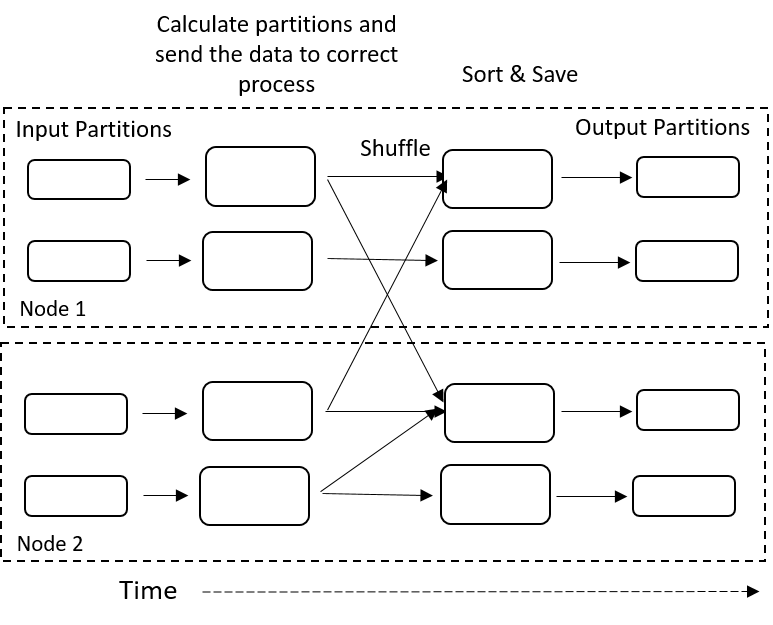
\includegraphics[width=0.8\columnwidth]{images/terasort_partition.png}
    \caption{Parallel sorting flow. Large boxes show the processes/tasks and small boxes are input files and output files.}
    \label{fig:tera_shuffle}
\end{figure}


\subsubsection{MPI}

In the MPI implementation the initial sampling is done in memory by choosing a subset of ranks. The samples are gathered to a single process to sort and create the partitioning. This partitioning is then broadcast to all the parallel tasks. The algorithm used send/receives along with iprobe to send the data to correct ranks. A chained send/receive topology in a ring is used, as shown in Fig~\ref{fig:fig_mpi_ring_send} to send the data. Unlike in Spark and Flink case lot of functionality had to be written in-order to get the algorithm working in a memory limited environment with file based sorting. Also to send the data efficiently the algorithm gathered large enough data set before sending it to the correct process. 

\begin{figure}
    \centering
    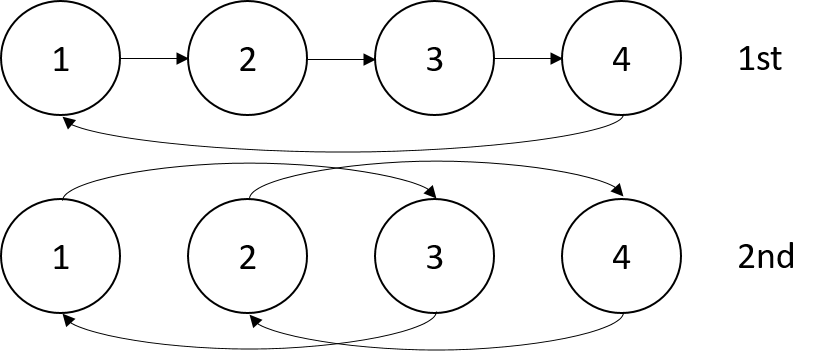
\includegraphics[width=0.55\columnwidth]{images/terasort_shuffle.png}
    \caption{MPI's data shuffling algorithm. Processes send and receive in a ring topology.}
    \label{fig:fig_mpi_ring_send}
\end{figure}


\subsubsection{Spark and Flink} 

Terasort can be implemented in Spark and Flink using the built-in capabilities of the platform. The data is loaded from HDFS cluster running in the same nodes. The data partitioning is done using the HDFS file system by reading the sample chunks in a single node; sorting them and writing the partitions back to HDFS. The sorting algorithm uses this partitioning to send the data to correct maps. The data is sorted using the sorting functions of Flink and Spark.

For Terasort, there was no apparent difference in the communication or the computation used by MPI, Flink or Spark. The MPI algorithm used send/receive operations which is essentially the mechanism used by Spark and Flink. Flink and Spark buffer the data internally while we buffered the data manually for sending using MPI.

\section{Evaluation} \label{evaluation}

The experiments were run on Juliet, which is an Intel Haswell HPC cluster. Up to 64 nodes were used for the experiments. These nodes have 24 cores (2 sockets x 12 cores each) per node. A node consists of 128GB of main memory and 56Gbps Infiniband interconnect and 1Gbps dedicated Ethernet connections. MPI experiments were conducted using TCP instead of Infiniband to make it comparable with Spark and Flink. For Flink and Spark experiments, the data was loaded from a HDFS cluster running on the same nodes. For MPI experiments data was copied to local storage in the nodes. For experiments we only used up to 20 cores in each node to reduce interference from other processes such as HDFS data nodes, Yarn, Flink TaskManager that run on these. MPI can utilize all the cores as it doesn't include additional processes.

\begin{figure*}[!htb]
    \centering
\begin{minipage}{.49\textwidth}
    \centering
    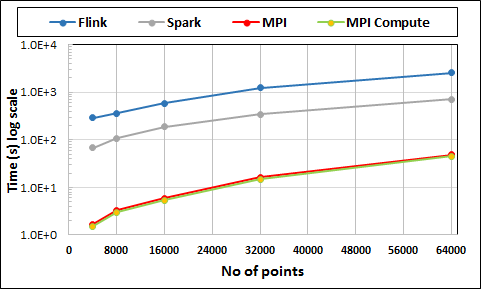
\includegraphics[width=0.95\columnwidth]{images/mds-points.png}
    \caption{MDS execution time on 16 nodes with 20 processes in each node with varying number of points}
    \label{fig:fig_mds_points}
\end{minipage}
\hspace{1.4mm}
\begin{minipage}{.49\textwidth}
    \centering
    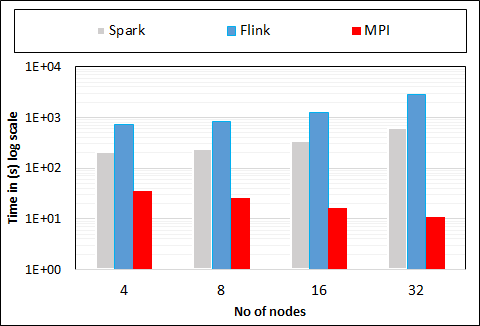
\includegraphics[width=0.95\columnwidth]{images/mds-nodes.png}
    \caption{MDS execution time with 32000 points on varying number of nodes. Each node runs 20 parallel tasks.}
    \label{fig:fig_mds_nodes}
\end{minipage}
\end{figure*}

For the experiments we ran MDS with a limited number of iterations with 5 temperature loops, 2 stress loops and 8 conjugate gradient iterations to limit the time required for experiments. Fig.~\ref{fig:fig_mds_points} shows time (displayed in log scale) for running MDS on 16 nodes with 20 parallel tasks in each node. The points are varied from 4000 to 64000. Flink performed very poorly as expected because it doesn't support nested iterations. Spark did considerably well compared to Flink but still proved much slower than MPI. This figure also shows the compute time of the MPI algorithm. It is evident that in MPI the communication overhead and other overheads when running the algorithm in parallel is minimal. Since the same parallel algorithm is implemented in Spark and Flink, this computing time provides a baseline for them as well. The large increase in time in Flink is caused by overheads introduced by the frameworks. 

Fig.~\ref{fig:fig_mds_nodes} Shown running the MDS algorithm with 32000 points on different number of nodes each having 20 parallel tasks. In MPI the running time decreases as expected while increasing the parallelism, and in Spark and Flink the running time increases with more nodes.  

\begin{figure*}[!htb]
\begin{minipage}{.49\textwidth}
    \centering
    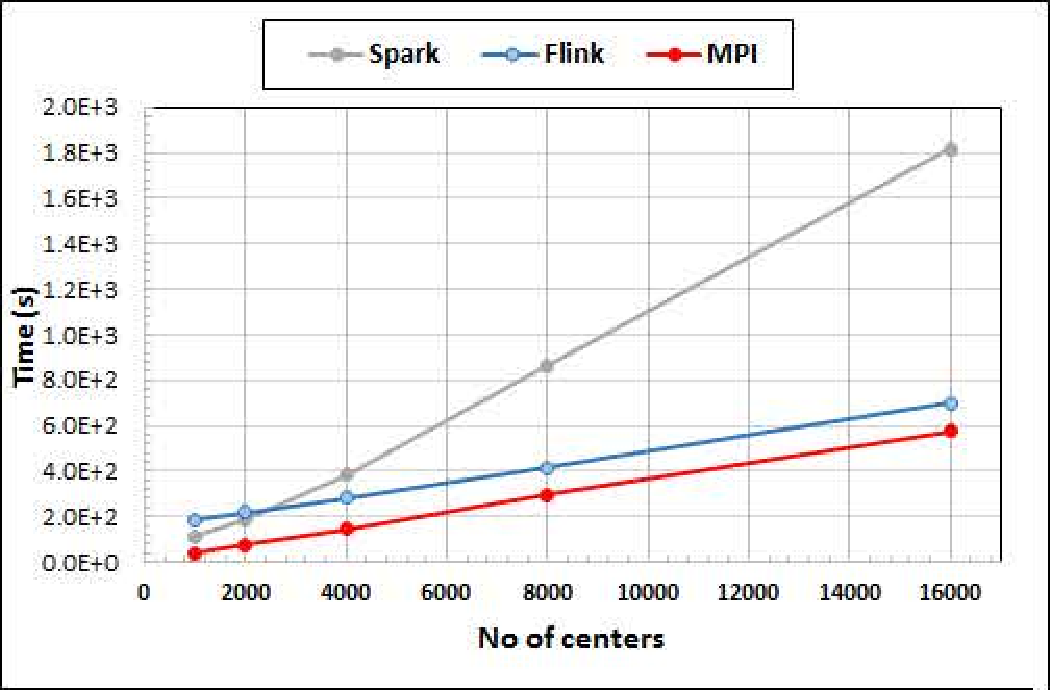
\includegraphics[width=0.95\columnwidth]{images/k-means-centers.pdf}
    \caption{K-Means execution time on 16 nodes with 20 parallel tasks in each node with 10 million points and varying number of centroids. Each point has 100 attributes.}
    \label{fig:fig_k_means_centroids}
\end{minipage}
\hspace{1.4mm}
\begin{minipage}{.49\textwidth}
    \centering
    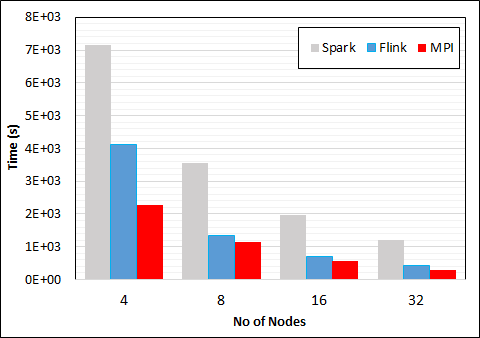
\includegraphics[width=0.95\columnwidth]{images/k-means-nodes.png}
    \caption{K-Means execution time on varying number of nodes with 20 processes in each node with 10 million points and 16000 centroids. Each point has 100 attributes.}
    \label{fig:fig_k_means_nodes}
\end{minipage}
\end{figure*}

\begin{figure*}[!htb]
\begin{minipage}{.49\textwidth}
    \centering
    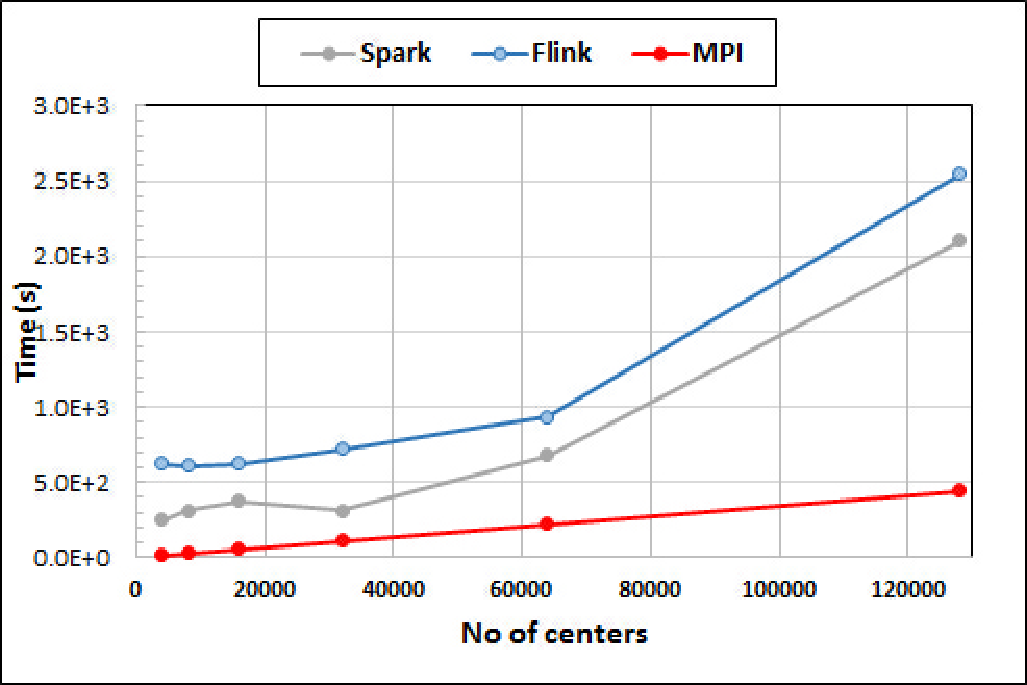
\includegraphics[width=0.95\columnwidth]{images/flink-small-centers.pdf}
    \caption{K-Means execution time on 8 nodes with 20 processes in each node with 1 million points and varying number of centroids. Each point has 2 attributes.}
    \label{fig:fig_k_means_small_centroids}
\end{minipage}
\hspace{1.4mm}
\begin{minipage}{.49\textwidth}
    \centering
    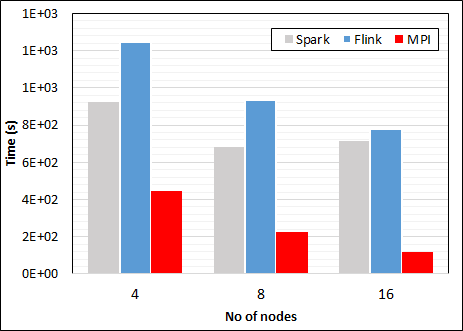
\includegraphics[width=0.95\columnwidth]{images/k-means-small.png}
    \caption{K-Means execution time on varying number of nodes with 20 processes in each node with 1 million points and 64000 centroids. Each point has 2 attributes.}
    \label{fig:fig_k_means_small_nodes}
\end{minipage}
\end{figure*}

We conducted two sets of experiments for the K-Means algorithm. In one experiment we used 10 million points each having 100 attributes (100 dimensions) and 10 iterations to calculate centers. In the next set we used 1 million points with 2 attributes and 100 iterations. The first test showed the amount of computation required is higher compared to the later experiment, which itself needed shorter computations and more communications because of the high number of iterations.

Fig.~\ref{fig:fig_k_means_centroids} shows the results of the 10 million point experiment in 16 nodes with varying number of centers. Flink worked comparatively better than Spark in this case and even performed closer to MPI performance. Fig.~\ref{fig:fig_k_means_nodes} shows the results of having 10 million points with 16000 centers and varying the number of nodes. Unlike in the MDS case, we saw decreases in time in all three frameworks when the parallelism increased. Fig.~\ref{fig:fig_k_means_small_centroids} shows the results of the 1 million point experiment in 8 nodes. The performance gap between MPI and Flink is wider in this case. Fig.~\ref{fig:fig_k_means_small_centroids} shows the same experiment with 64000 centers and varying number of nodes. As the parallelism increased again, MPI performed better but Flink did not scale well.

\begin{figure}
    \centering
    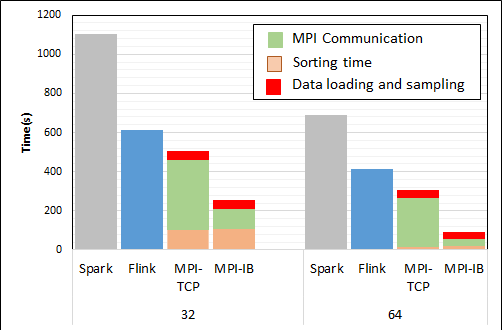
\includegraphics[width=0.9\columnwidth]{images/terasort-bar2.png}
    \caption{Terasort execution time in 64 and 32 nodes. Only MPI shows the sorting time and communication time as other two frameworks doesn't provide a viable method to accurately measure them. Sorting time includes data save time. MPI-IB - MPI with Infiniband}
    \label{fig:terasort_time}
\end{figure}

Fig.~\ref{fig:terasort_time} shows the run time of sorting 1 Terabyte of data in 64 nodes with all three frameworks. Because we are mainly comparing the in-memory performance of the algorithms, we used sufficient nodes so that we can do the sorting in-memory without using the disks. As such the largest time of the algorithm was spent on shuffling the data across multiple processes. In this case all the frameworks performed reasonably well and produced results closer to each other, although the MPI Infiniband results are significantly faster than other approaches. For 32 node test the memory was insufficient and the program had to use the disk to perform the sorting. The MPI-IB test shows that MPI with Infiniband performed best in transferring the data quickly. For 32 node MPI case we noticed that Java garbage collection was affecting the performance. This is an initial investigation, which we will extend later.

\begin{figure}
    \centering
    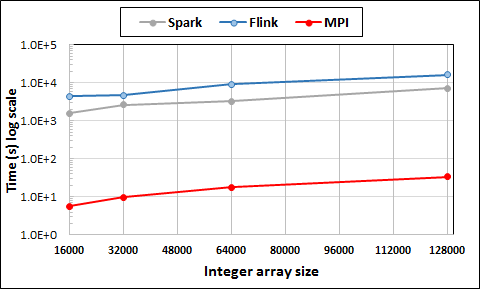
\includegraphics[width=0.9\columnwidth]{images/reduce.png}
  \caption{Reduce operation time with 640 parallel tasks in 32 nodes. Integer array with different sizes is used for the reduce operation.}
    \label{fig:reduce_time}
\end{figure}

A micro benchmark was conducted to measure the reduce operation communication time in the three frameworks and its results are shown in Fig.~\ref{fig:reduce_time}. The experiment was conducted in 32 nodes with 20 parallel tasks in each node having 640 parallel tasks. Integer array of varying sizes is used for the reduction operation, which was conducted several times in an iteration to calculate the average time. It is clear from the graph that there is a large difference in time between Flink and MPI.

\section{Discussion} \label{discussion}

MDS is the most complex algorithm among the three algorithms considered here. We have encountered many inefficiencies of Spark and Flink while implementing the algorithm. For Flink the biggest inefficiency was its inability to support nested loops. This leads to a very laborious implementation where we save the intermediate data to file system at each iteration in the outer two loops. Also the way Flink is designed means it needs to read the input files each time it does the iterations, adding to the overhead. The main inefficiency in the Spark MDS implementation was caused due to the lack of all-to-all collective operations. Using a reduce operations followed by a broadcast operation added couple of overheads to the algorithm. 

K-Means showed some interesting characteristics with the three frameworks we used. In parallel K-Means, the communication cost is a direct function of the number of centroids involved and it doesn't depend on the number of points. With increased number of points, the computation time increases, but the communication time remains the same. When using the 10 million data set it was evident that Flink performed close to MPI, and when using the 1 million data set with 100 iterations, the performance gap widened. We concluded that Flink-like frameworks need improvements in communication algorithms used for transferring data to scale to larger nodes when communication requirements are high. Most of the practical clustering problems do not have hundreds of thousands of clusters. This means K-Means can perform equally better in Flink or spark for practical data analytics tasks.

For Terasort, both Flink and MPI displayed comparable performance results. The communication in Terasort involves transferring large amounts of data among the nodes. Ring-like topologies produce the best results for throughput in such bulk transfers since they effectively use the networks in all the nodes at the same time as evident by the good performance in MPI algorithm. Since Flink and Spark do the asynchronous point to point communications, they both saw the similar performance to MPI. Writing the MPI algorithm required time and effort and for such tasks involving transferring large amount of data Flink and Spark can be better choices given the ease of use. 

The experiments showed an interesting observation where big data frameworks doesn't scale well for algorithms with high frequency of communicate and compute regions. Also it was evident that Spark performed better than Flink when there was high frequency of communication and computation regions. Algorithms with longer computation and communication times performed well in Flink compared to Spark.

The micro-benchmarks show there is a big difference in communication times for collective communications between MPI and the big data platforms. The primary reason is that, MPI has implemented very efficient collective communication algorithms while Flink and Spark rely on point to point connections.

\section{Related Work} \label{related}

An immense amount of research is being done on improving performance and resource utilization in both the Big Data and HPC communities. Research on improving performance of Spark is being done in Project Tungsten~\cite{tungsten} where they aim to improve performance by introducing its own memory management and cache handling system. Even though we mainly talked about Spark and Flink, there are a large number of frameworks utilized in the Big Data community, each having pros and cons over each other. Pregal~\cite{malewicz2010pregel}, Apache Hama~\cite{seo2010hama} and Apache Giraph~\cite{Giraph} are frameworks that were developed around the BSP model. There are also numerous distributed graph processing frameworks, including GraphX~\cite{gonzalez2014graphx}. Doekemeijer et al.~\cite{doekemeijer2014survey} compare and contrast many distributed graph processing frameworks. Much research has also been done on integrating HPC technology into big data frameworks to improve performance. Lu et al. ~\cite{lu2013high} integrate RDMA technology to improve performance of Hadoop. Hpc-abds ~\cite{7152592} discusses and summarizes HPC and Big data convergence.   

Owing to the increasing popularity of machine learning algorithms, most Big Data frameworks provide machine learning libraries. Mlib~\cite{meng2016mllib} is built on top of Spark and offers a wide variety of machine learning algorithms. FlinkML~\cite{carbone2015lightweight} is the requisite library for Flink. Intel Data Analytics Acceleration Library (DAAL)~\cite{inteldaal} from Intel has been tuned for Intel architecture; it provides functions for deep learning, classical machine learning, etc. Tensorflow ~\cite{abadi2016tensorflow} is a library developed at Google. Algorithms developed using TensorFlow can be executed in a wide variety of heterogeneous systems that range from mobile devices to supercomputers. h2o~\cite{h2omachinelear} is a machine learning framework that supports Spark and Hadoop with simplified APIs for ease of use. Apache Mahout~\cite{owen2012mahout} remains another popular framework originally developed to support machine learning on top of Hadoop and later expanded to support other frameworks.

There is a lot of focus today on comparing HPC technology with Big Data technology in order to understand pros and cons of each. These comparisons contribute towards the HPC/Big Data convergence by identifying areas that can be improved in each technology domain. The authors have studied about HPC/Big Data convergence~\cite{fox1858big} in more detail. Reyes-Ortiz et al. ~\cite{reyes2015big} compare Spark and MPI/OpenMP on Google Cloud platform to compare and contrast performance, data management, etc. between the two frameworks. Liang et al. ~\cite{liang2014performance} compare DataMPI~\cite{lu2014datampi}, which is an extension of MPI developed to execute Hadoop-like Big Data jobs, with Spark and Hadoop using BigDataBench~\cite{wang2014bigdatabench}. The authors previously studied factors that affect performance of Java machine learning applications in Multicore HPC Clusters~\cite{ekanayakejava}.

TeraSort is a popular sorting algorithm that can be used to measure I/O performance of frameworks. Lu et al.~\cite{lu2014datampi} use Terasort to compare DataMPI to Hadoop and Marcu et al.~\cite{marcu2016spark} use Terasort to compare Spark and Flink. MDS is a popular method used for dimension reduction, DA-MDS~\cite{bae2010multidimensional} used in this paper is a Deterministic Annealing approach to MDS which can outperform other MDS implementations. 

\section{Conclusion \& Future Work} \label{conclusion}
The three algorithms presented here show different performance across the three frameworks for the algorithms considered. MPI performed the best in all three algorithms, but it was the hardest to program among the three. A reasonable person can pick Spark or Flink over MPI simply due to the trade off of performance vs ease of use. Flink and Spark performed well on the Terasort algorithm and K-Means with minimal coding efforts while performing poorly on the more sophisticated MDS algorithm. There are large number of machine learning algorithms that are in the range of K-Means and Terabytesort complexity and they can be efficiently implemented in these platforms. For more complex algorithms these frameworks needs to be improved to support the algorithm requirements. For example, Flink and Spark require efficient communication algorithms to scale complex machine learning algorithms that require tight synchronizations and collective communications. We are working on to improve the performance of Flink and Spark by improving their communication algorithms. 

% needed in second column of first page if using \IEEEpubid
%\IEEEpubidadjcol

% An example of a floating figure using the graphicx package.
% Note that \label must occur AFTER (or within) \caption.
% For figures, \caption should occur after the \includegraphics.
% Note that IEEEtran v1.7 and later has special internal code that
% is designed to preserve the operation of \label within \caption
% even when the captionsoff option is in effect. However, because
% of issues like this, it may be the safest practice to put all your
% \label just after \caption rather than within \caption{}.
%
% Reminder: the "draftcls" or "draftclsnofoot", not "draft", class
% option should be used if it is desired that the figures are to be
% displayed while in draft mode.
%
%\begin{figure}[!t]
%\centering
%\includegraphics[width=2.5in]{myfigure}
% where an .eps filename suffix will be assumed under latex, 
% and a .pdf suffix will be assumed for pdflatex; or what has been declared
% via \DeclareGraphicsExtensions.
%\caption{Simulation Results}
%\label{fig_sim}
%\end{figure}

% Note that IEEE typically puts floats only at the top, even when this
% results in a large percentage of a column being occupied by floats.


% An example of a double column floating figure using two subfigures.
% (The subfig.sty package must be loaded for this to work.)
% The subfigure \label commands are set within each subfloat command, the
% \label for the overall figure must come after \caption.
% \hfil must be used as a separator to get equal spacing.
% The subfigure.sty package works much the same way, except \subfigure is
% used instead of \subfloat.
%
%\begin{figure*}[!t]
%\centerline{\subfloat[Case I]\includegraphics[width=2.5in]{subfigcase1}%
%\label{fig_first_case}}
%\hfil
%\subfloat[Case II]{\includegraphics[width=2.5in]{subfigcase2}%
%\label{fig_second_case}}}
%\caption{Simulation results}
%\label{fig_sim}
%\end{figure*}
%
% Note that often IEEE papers with subfigures do not employ subfigure
% captions (using the optional argument to \subfloat), but instead will
% reference/describe all of them (a), (b), etc., within the main caption.


% An example of a floating table. Note that, for IEEE style tables, the 
% \caption command should come BEFORE the table. Table text will default to
% \footnotesize as IEEE normally uses this smaller font for tables.
% The \label must come after \caption as always.
%
%\begin{table}[!t]
%% increase table row spacing, adjust to taste
%\renewcommand{\arraystretch}{1.3}
% if using array.sty, it might be a good idea to tweak the value of
% \extrarowheight as needed to properly center the text within the cells
%\caption{An Example of a Table}
%\label{table_example}
%\centering
%% Some packages, such as MDW tools, offer better commands for making tables
%% than the plain LaTeX2e tabular which is used here.
%\begin{tabular}{|c||c|}
%\hline
%One & Two\\
%\hline
%Three & Four\\
%\hline
%\end{tabular}
%\end{table}


% Note that IEEE does not put floats in the very first column - or typically
% anywhere on the first page for that matter. Also, in-text middle ("here")
% positioning is not used. Most IEEE journals use top floats exclusively.
% Note that, LaTeX2e, unlike IEEE journals, places footnotes above bottom
% floats. This can be corrected via the \fnbelowfloat command of the
% stfloats package.




% use section* for acknowledgement
\section*{Acknowledgment}
This work was partially supported by NSF CIF21 DIBBS 1443054 and NSF RaPyDLI 1415459. We thank Intel  for their support of the Juliet system, and extend our gratitude to the FutureSystems team for their support with the infrastructure.

% Can use something like this to put references on a page
% by themselves when using endfloat and the captionsoff option.
\ifCLASSOPTIONcaptionsoff
  \newpage
\fi



\balance
\bibliography{bibtex/ref.bib}{}
\bibliographystyle{IEEEtran}





% that's all folks
\end{document}


